\documentclass[conference]{IEEEtran}
\IEEEoverridecommandlockouts
% The preceding line is only needed to identify funding in the first footnote. If that is unneeded, please comment it out.
\usepackage{cite}
\usepackage{amsmath,amssymb,amsfonts}
\usepackage{algorithmic}
\usepackage{graphicx}
\usepackage{textcomp}
\usepackage{xcolor}
\def\BibTeX{{\rm B\kern-.05em{\sc i\kern-.025em b}\kern-.08em
    T\kern-.1667em\lower.7ex\hbox{E}\kern-.125emX}}
\begin{document}

\title{Challenges Encountered in Developing GitHub Actions and its Ecosystem\\
}

\author{
\begin{tabular}{@{}ll}
Name of student 1: Kardo Marof \\
Name of student 2: Saif Sayed \\
\\
Proposed academic supervisor's name (leave blank if you do not have an academic supervisor): Linda Erlenhov \\
Have your proposed academic supervisor \textbf{clearly} stated that he/she will supervise you: YES \\
\\
Will the thesis work be conducted in collaboration with an external organization: NO \\
If yes, is your supervisor aware of the external organization and the contact person/advisor: YES / NO
\end{tabular}
}

\maketitle

                                                                        %%% INTRODUCTION %%%
\section{Introduction}
    Continuous Integration (CI) has become an integrated part of collaborative software development and DevOps practices. CI automates the quality of code checks, tests and integration of code changes in collaborative environments. The benefits of CI brings early detection of issues, fast feedback loops, increased code quality, reduced integration risks and continuous improvements. Famous examples of CI services include Jenkins, Travis, CircleCI and GitLab CI/CD \cite{dabbish2012social}. GitHub Actions (abbreviated as GHA) was introduced to the public in 2019 as an alternative CI service for GitHub repositories. GitHub introduced its marketplace for sharing automation tools in an effort for developers to reuse workflow components \cite{saroar2023developers}. \\ 

    The so called "Actions" refers to automated workflows triggered by specific events within a repository, including committing changes, opening pull requests, or creating new branches. These workflows streamline development processes by automating tasks and enhancing efficiency. GitHub's integration of GHA allows developers to define custom task sequences in response to events, simplifying collaboration and promoting a seamless development experience \cite{chandrasekara2021getting}. \\



    The growing popularity of GHA is immense, with on average more than 20 million GitHub Action minutes used per day in 2023. This growth leads to a 169\% increase in the usage of automating tasks in public projects,  pipelines and more\cite{github2023octoverse}. Given its popularity,  the increasing usage of GHA has lead to an emergence of its own ecosystem \cite{decan2022use}.  According to Decan et al. \cite{decan2022use}, the growing ecosystem of GHA bears similarities to reusable software libraries distributed by package managers such as npm, Cargo, RubyGems, Maven and PyPI among others. Where these ecosystems are well known to suffer from variety of issues such as obsolescence, dependency issues, breaking changes and security vulnerabilities to name a few\cite{decan2022use}. The authors go on to state "\textit{The GHA ecosystem is likely to suffer from very similar issues and these issues will continue to become more important and more impactful, as the number of reusable Actions continues to grow at a rapid pace.}"\\

    Given the concerns surrounding the GHA ecosystem, it is self-evident that developers will experience the effects of these issues.  Moreover, it's worth noting that not all Actions are available on the GitHub marketplace. Many developers create and maintain their own Actions within local repositories, without making them available on the marketplace. The authors  conducted an analysis of prevalent automation practices on GitHub and discovered that 43.9\% of repositories in their dataset reflected this behavior \cite{decan2022use}.\\

    Due to its novelty, there is limited understanding of the challenges faced when implementing GHA.  
    Therefore,  by systematically analysing StackOverflow posts, GitHub Discussions threads, tags, and other pertinent repositories, alongside the utilisation of database queries and APIs, we aim to quantitatively examine the questions, topics, and answers surrounding GHA. This endeavor not only facilitates the clarification of prevalent issues but also provides insights into potential solutions and areas requiring further research and development within the GHA landscape.\\

    Through this research, we intend to answer the following questions:\\


    \textbf{RQ1: What factors cause developers to rely on locally maintained Actions within their repositories, as opposed to utilizing Actions available on the GitHub Marketplace?}\\\\
    We selected RQ1 in order to distinguish the problems faced between locally maintained and marketplace Actions. It is not currently known the exact factors that contribute to this distribution. There are also workflows that utilise both action types and knowing which action types are more locally maintained opposed to others, will give great insight into the decision making of designing and developing a workflow. \\

 \textbf{RQ2: In what ways do the key issues encountered in GitHub Actions (GHA) parallel those found in other software ecosystems?}\\\\
    This research question is inspired by the concerns raised by Decan \cite{decan2022use}, as previously mentioned. The objective is to compile a list of current issues prevalent in reusable software libraries distributed via package managers and draw parallels with our research findings. This comparative analysis aims to determine whether these concerns are indeed applicable to the GHA ecosystem. If similarities are found, it will aid in identifying effective solutions previously implemented in other ecosystems to address these issues. Subsequently, these solutions can be adapted for the GHA ecosystem to prevent the escalation of such problems in the future.



                                                                        %%% RELATED WORK %%%

\section{Related Work}
    After just 18 months since its official release, previous research has demonstrated a notable surge in the popularity of GHA, leading to a gradual shift away from conventional CI/CD services in GitHub repositories \cite{golzadeh2021rise}. Unlike conventional CI/CD services, GHA assists the software development processes by improving code reviews, team communication and internal repository management in addition to automating the build and test procedures of software \cite{chandrasekara2021hands}. As previously mentioned, this emerging popularity on the use of GHA and the increasing number of reusable Actions that can be found on its marketplace led GHA to be considered similar to popular reusable software libraries distributed by package managers such as npm, Cargo, RubyGems, Maven and PyPI and so on. However, this also means GHA is more likely to face similar problems that are currently encountered by these reusable libraries \cite{decan2022use}. Consequently, this would increase the chances of failure when building GitHub workflows in GitHub repositories leading to unsuccessful deployment of software packages. \\

    According to Decan \cite{decan2022use}, the GHA ecosystem deserves to be studied as all other reusable software ecosystems that have made progress in finding issues related to them. Since GHA is a new emerging ecosystem, there is a lack of research and studies that have been carried out to identify the challenges and issues that are encountered in GHA. The authors point out that the GHA ecosystem is exposed to similar challenges, such as obsolescence \cite{decan2018evolution} \cite{cogo2021deprecation}, dependency issues \cite{decan2019empirical} \cite{soto2021comprehensive} \cite{decan2019package}, breaking changes \cite{dietrich2019dependency}\cite{decan2018impact} and security vulnerabilities \cite{zimmermann2019small} \cite{kula2018developers}, that are encountered in well-researched ecosystems. This section aims to briefly describe some of the issues pointed out above, using findings from related literatures, that are likely to appear in GHA.

    \subsection{Obsolescence}
        Software codes are regularly updated to add features, fix bugs, etc. Sometimes functions or parts of code become deprecated meaning they are outdated and no longer used; this usually happens after a long period of time, when parts of the software code are replaced by an improved version. Generally, it is a good practice to avoid using deprecated code. Through the findings of Cogo et al. \cite{cogo2021deprecation}, deprecated code used in npm packages has shown to give rise to risks such as incompatibility between two different dependant libraries, presence/absence of features, bugs, security vulnerability and more. Cox et al. \cite{cox2015measuring} found that deprecated systems are four times more likely to suffer from security issues and backward incompatibilities than systems that are up-to-date. In the context of GHA, there is a high possibility that a significant amount of code used within the workflow is deprecated which may consequently lead to build failures.

    \subsection{Dependency Issues}
        Software systems are usually developed using pre-existing and reusable packages such as modules, components, libraries, etc \cite{decan2019empirical}\cite{soto2021comprehensive}. Consequently, this leads to a large extent of dependencies between the reused packages and the original software code. According to Dietrich et al. \cite{dietrich2019dependency}, software developers struggle to choose which versions of a given package to use and that a handful number of software systems encounter runtime version conflicts due to incompatibility with the versions of other dependant packages. Actions and workflows that depend on jobs from other Actions might fall on a similar pitfall of runtime version conflicts and possibly other dependency issues. Valenzuela-Toledo and Bergel \cite{valenzuela2022evolution} claim they have found instances of workflows where modifications were made to update the version of the tool/software being used in a particular job (e.g., Figure 1 \cite{valenzuela2022evolution}  ).

\begin{figure} [h]
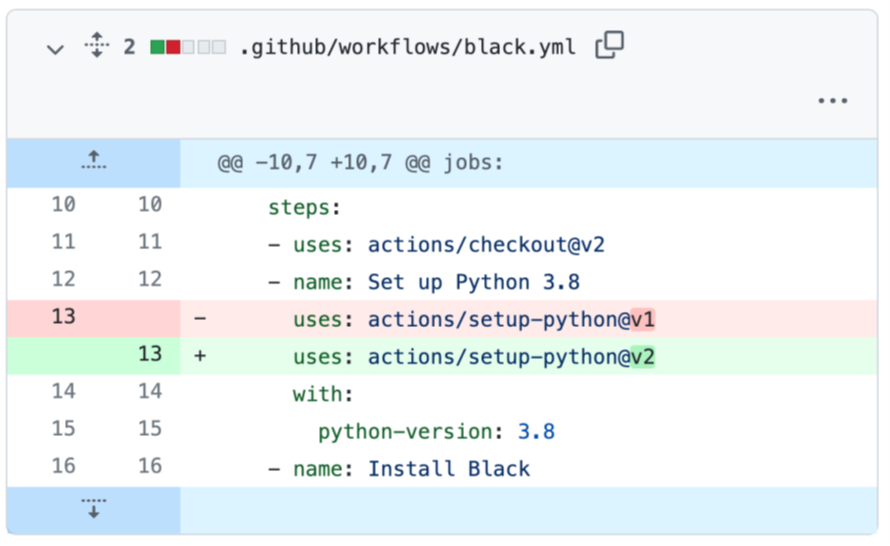
\includegraphics[width=0.5\textwidth]{Figure 1.png}
\caption{Modifying python version \cite{valenzuela2022evolution} }
\end{figure}

    \subsection{Security Vulnerabilities}
        Software that depends on open source and free reusable libraries provided by package managers like npm are more likely to be exposed to security vulnerabilities. To quote Zimmermann et al. \cite{zimmermann2019small}, they mention the following: \\

        \textit{"The open nature of npm has boosted its growth, providing over 800,000 free and reusable software packages. Unfortunately, this open nature also causes security risks, as evidenced by recent incidents of single packages that broke or attacked software running on millions of computers.”} \\

        According to Koishybayev et al. \cite{koishybayev2022characterizing}, one example of a similar attack using the GHA ecosystem is to perform deployments based on the attacker’s code by triggering a misconfigured workflow through a new pull request. Since GHA consists of many open-source reusable Actions, workflow and GHA developers need to be extra careful on choosing what packages they depend on for building jobs. It is a good practice to depend on first-party packages and packages from trustworthy maintainers \cite{zimmermann2019small}. \\

        Saroar et al. \cite{saroar2023developers} mentions that even though the GHA platform provides a marketplace for sharing and reusing open-source Actions, there are still many repositories that prefer to maintain their own GitHub workflows. Although, the survey analysis conducted by the authors resulted in identifying several challenges developers face when using their own customised YAML files.  The results indicated that developers found YAML files to be: (i) confusing and error-prone; (ii) difficult to test and debug; and (iii) hard to follow indentation rules. Another study by Valenzuela-Toledo and Bergel \cite{valenzuela2022evolution}  showed that modifications to GitHub workflows are made to correct YAML syntax and debug GHA workflows which is in line with the previous study \cite{saroar2023developers}. The survey also revealed some challenges GitHub users face using the Marketplace where 7 out of 25 participants found it difficult to search for products and hard to check product quality (see Figure 2). Saroar et al. \cite{saroar2023developers} quotes one of the participants from the survey: \\

\textit{"Marketplace does not provide an effective way to filter and sort based on quality, version, contributions, etc."}\\

\begin{figure} [h]
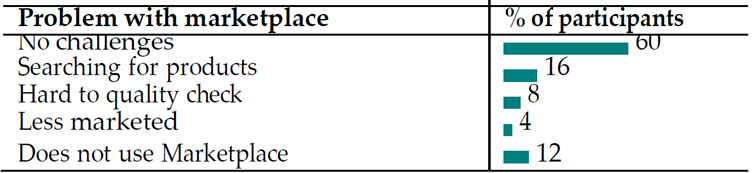
\includegraphics[width=0.5\textwidth]{Table 1.png}
\caption{Challenges found when using GitHub Marketplace \cite{saroar2023developers} }
\end{figure}

                                                                        %%% RESEARCH MOTHODOLOGY %%%

\section{Research Methodology}
    With this study we aim to answer some of the challenges and problems developers face when building GHA. Our goal is to evaluate whether similar challenges and issues from well-researched reusable libraries can be spotted in the GHA ecosystem.\\

    In this section, we describe the research questions we are trying to answer and the research strategies which will be implemented to facilitate our explorative study. Additionally, we would like to emphasize that we are employing a mixed method study, utilising different data collection and analysis methods that will be described and motivated after each research question. Finally, we identify and explain the limitations relevant to our research.

    \subsection{Research questions and methodology}


        \textbf{RQ1: What factors developers to rely on locally maintained Actions within their repositories, as opposed to utilising Actions available on the GitHub marketplace?}\\

        \textbf{Research Method:} Survey\\
            
        This research question is answered by determining whether developers prefer to build their own GitHub workflows or reuse GitHub actions from the marketplace. Additionally, it aims to explain the reasons behind the observed differences between these approaches.\\

        To address RQ1, we plan to conduct surveys of individuals from a large group of GitHub users utilizing GHA across the internet. A questionnaire is designed to obtain qualitative and statistical data about their preferences. Linåker et al. \cite{linaker2013guidelines} claim that conducting an online survey makes it possible to collect data for a large population efficiently by generalizing our findings based on a sample. Moreover, surveys are suitable for collecting numerical data which would allow us to analyse responses numerically to identify patterns and trends in our results \cite{fowler2009survey}. We believe utilizing this methodology is time and cost effective compared to other research methodologies; since surveys can be administered remotely, eliminating the need for face-to-face interactions, and reducing operational costs.\\

        \subsubsection{\textbf{Data Collection}}
            To administer online surveys, the target audience will be active GitHub users engaged in software development and GitHub Actions (GHA) workflows. Instrumentation entails designing a questionnaire to collect demographic information, usage patterns of GHA, and factors influencing the selection of Actions. The aim is to collect responses from at least 50 participants. This procedure will include distributing surveys through GitHub platforms, developer forums, and social media channels. The time schedule encompasses a one-month plan to design, distribute, and collect responses efficiently.\\

        \subsubsection{\textbf{Data Analysis}}
            In the analysis phase, the intent is to utilize both descriptive and inferential statistical techniques to rigorously scrutinize the survey data.  This entails establishing specific criteria for analysis, including the definition of metrics such as the frequency of marketplace action usage, rationales underlying action selection, and the perceived advantages and disadvantages associated with these selections. Moreover, the evaluation process will involve a meticulous examination of emerging trends and the identification of factors shaping distribution patterns.\\

        \textbf{RQ2: In what ways do the key issues encountered in GHA parallel those found in other software ecosystems?}\\

        \textbf{Research Method:} Repository Mining and Interview\\

        We are already aware of the problems encountered in other ecosystems. Our goal is to identify similar challenges and/or issues within the GHA ecosystem and evaluate the impact of these problems. Additionally, we want to investigate what are the challenges developers face while implementing workflows.\\

       To address RQ2, we plan to carry out repository mining and interviews. Through repository mining, we can collect vast amounts of data from relevant software repositories using GHA. We can also automate the process of mining data by developing scripts and easing the process of going through multiple repositories \cite{chaturvedi2013tools}. By combining repository mining with semi-structured interviews would allow us to compare our quantitative data with qualitative data obtained from the interviews. Thus, we can validate our findings from one methodology against the other; this would strengthen the credibility and reliability of our research findings. Moreover, through interviews, we might also come across further problems encountered by developers. According to Rigby and Storey \cite{rigby2013understanding}, interviews can help identify topics that are not well-documented in software repositories, such as the reasons behind code changes and developer’s experiences.\\

        \subsubsection{\textbf{Data Collection}}
            The first methodology will be to utilise APIs and database queries to collect relevant data from StackOverflow, GitHub Discussions, and other pertinent repositories via Repository/Data Mining. The data of interest will pertain to challenges within the scopes of obsolescence, dependency issues, breaking changes and security vulnerabilities. 
            The second methodology will be to conduct semi-structured interviews with developers experienced in GHA usage and are actively devoloping. To recruit participants, we aim to utilise our existing network within Volvo Group Trucks Technology and aim to interview 10 team leaders involved in Software Development utilising GHA in their environments, upon agreement. The procedure will be to Develop interview protocols focusing on specific topics related to the challenges. The time schedule is to Allocate 1 month for data collection, including both repository/data mining and interviews.\\

        \subsubsection{\textbf{Data Analysis}}
            In our data analysis approach, we will employ repository mining techniques to analyze patterns and trends in StackOverflow posts, GitHub Discussions threads, and repository data obtained through APIs and database queries. Quantitative analysis will encompass descriptive statistics such as mean and visualization methods including histograms and scatter plots. Qualitative analysis techniques will be utilized to analyze interview transcripts and identify recurring themes. Moreover, in Mining Software Repositories (MSR), we will extract and analyze metrics such as code churn and complexity. We may also explore the application of machine learning methods, with detailed descriptions provided to ensure transparency and repeatability. Overall, our approach aims to provide a comprehensive understanding of the challenges in the GHA ecosystem parallel to other software ecosystems.\\

        These methods ensure a systematic approach to address each research question effectively.\\

    \subsection{Time Plan}
        The table bellow gives a high level overview of the time plan. A SCRUM framework will be in use throughout the management of the research. 
        \begin{table}[h]
            \centering
            \caption{Project Sprint Timeline}
            \label{tab:sprint_timeline}
            \begin{tabular}{|c|p{0.7\linewidth}|}
            \hline
            \textbf{Sprints} & \textbf{Activities} \\ \hline
            1 and 2 & Design base structure for data collection:
            \begin{itemize}
                \item Surveys
                \item Interview questions
                \item API scripts
                \item Database Queries
                \item Document and write the literature
            \end{itemize} \\ \hline
            3 and 4 & Collect data based using the instruments designed in sprints 1 and 2:
            \begin{itemize}
                \item Conduct interviews
                \item Send out surveys
                \item Run and gather data from API calls and queries
                \item Document and write the literature
            \end{itemize} \\ \hline
            5 and 6 & Analyse the data collected from sprints 3 and 4:
            \begin{itemize}
                \item Detect patterns
                \item Identify key factors
                \item Draw conclusions
                \item Document and write the literature
            \end{itemize} \\ \hline
            7 and 8 & Refine and finalize the analysis and ensure the literature is clear and concise. \\ \hline
            \end{tabular}
        \end{table}

    \subsection{Threats to Validity}
        In this section, we discuss the limitations and threats to
        validity and how we can mitigate them.\\

        \textbf{External Validity:} Since our repository mining procedure is supposed to collect data from diverse GitHub repositories with different implementation of workflows, programming languages and size of the project, the results we obtain might differ depending on these factors and our findings can’t be generalized for all types of GitHub projects. However, it is possible to group the projects based on their size, programming language, etc. After grouping the projects, we could try to analyse data from each group and identify a common trend between the results to generalize our findings.\\

        \textbf{Internal validity:} Collecting data through online surveys carries some risks and may result in anomalies in our results. Specifically, distributing surveys via social media can lead to invalid responses, and we may also face challenges in obtaining a sufficient number of responses to draw meaningful conclusions. To mitigate these potential limitations, we can consider distributing surveys through highly maintained development platforms or reaching out to potential companies in person. \\

	\textbf{Construct Validity:} The questionnaire, we are planning to use as our survey instrumentation, might have errors or inconsistencies. The formulated questions might be unclear, ambiguous and/or irrelevant. We could address this risk by adhering to a well-defined criterion for formulating questionnaires. Additionally, we could conduct pilot testing to validate our survey instrument.

							    %%% ACKNOWLEDGEMENT %%%

\section{Acknowledgement}

         This proposal is the collaborative effort of Kardo Marof and Saif Sayed, with guidance from our thesis supervisor, Linda Erlenhov. Marof's contributions include the Introduction section, as well as the sub-sections on Data Collection and Data Analysis within the Research Methodology section. Sayed, on the other hand, contributed to the Related Works section, the description of the Research Questions, the motivation behind the selected methodologies, and the identification of Threats to Validity within the Research Methodology section.


                                                                        %%% REFERENCES %%%

\bibliographystyle{unsrt}
\bibliography{references}

\vspace{12pt}
\end{document}
